% !TEX root = ../Noctua_Pflichtenheft.tex

% Chapter4
\chapter{Produktfunktionen}\label{chapter:Produktfunktionen}

\section{Funktionen der Marktszustandsbestimmung}

\begin{minipage}[t]{\textwidth}
/F010/ \textbf{Vergangene Marktzust�nde bestimmen}

\begin{center}

\begin{tabular}{ | l | p{10cm} |}
\hline 
Beschreibung & Es sollen historische Marktzust�nde (innerhalb der letzten Jahre) auf transparenten
Aktienm�rkten, f�r die ein ausreichender Datenbestand vorhanden ist, automatisch bestimmt
werden. Sollten sich verschiedene gro�e M�rkte entgegen der Erwartung entsprechend
unterschiedlich verhalten, dass diese keiner einheitlichen Analyse unterzogen werden k�nnen,
soll prim�r der US-amerikanische Aktienmarkt untersucht werden. Hierbei handelt es sich um
eine Gruppierung von Zeitabschnitten nach gemeinsamen Kriterien.\\  \hline
Akteure & System \\ \hline
Teilsystem & Algorithmus \\ \hline
Ziel & Ermittelung von Klassen f�r Marktzust�nde. \\ \hline
Vorbedingungen & - \\ \hline
Nachbedingungen & - \\ \hline

\end{tabular}

\end{center}
\end{minipage}\\[4ex]

\begin{minipage}[t]{\textwidth}
/F020/ \textbf{Aktuellen Marktzustand bestimmen}

\begin{center}

\begin{tabular}{ | l | p{10cm} |}
\hline 
Beschreibung & Dabei soll darauf geachtet werden, dass f�r eine fr�he Erkennung m�glicherweise nur ein Teil
der Daten vorhanden ist, die f�r die historische Analyse herangezogen werden k�nnen.\\  \hline
Akteure & System \\ \hline
Teilsystem & Algorithmus \\ \hline
Ziel & Zuordnung des aktuellen Marktzustandes zu einem bereits bekannten. \\ \hline
Vorbedingungen & /F010/ Vergangene Marktzust�nde bestimmen \\ \hline
Nachbedingungen & - \\ \hline

\end{tabular}

\end{center}
\end{minipage}\\[4ex]

\section{Funktionen des Trading-Algorithmus}

\begin{minipage}[t]{\textwidth}
/F110/ \textbf{Trends erkennen}

\begin{center}

\begin{tabular}{ | l | p{10cm} |}
\hline 
Beschreibung & Durch \glspl{ma} soll es m�glich sein, Trends in Aktienkursen zu identifizieren. Dazu
kommen verschiedene Crossover-Verfahren (double- / triple-crossover) oder Indikatoren, wie
der MACD (Moving Average Convergence Divergence) in Frage. Es soll eine statistisch
m�glichst profitable Variante hierf�r gefunden werden, die aufscheinende nachhaltige Trends
m�glichst g�nstig erkennt.\\  \hline
Akteure & System \\ \hline
Teilsystem & Algorithmus \\ \hline
Ziel & Fr�hzeitige m�glichst profitable Erkennung von Trends. \\ \hline
Vorbedingungen & - \\ \hline
Nachbedingungen & - \\ \hline

\end{tabular}

\end{center}
\end{minipage}\\[4ex]

\begin{minipage}[t]{\textwidth}
/F120/ \textbf{\gls{ma}-Dauer bestimmen}

\begin{center}

\begin{tabular}{ | l | p{10cm} |}
\hline 
Beschreibung & Je nachdem, wie lange ein Trend andauert, bedingt eine Trenderkennung andere \gls{ma}(-Paare)
mit unterschiedlichen Laufzeiten. Aus zum Beispiel bew�hrten Wertepaaren oder adaptiven Methoden sollen
automatisch die optimalen Laufzeiten gew�hlt werden.\\  \hline
Akteure & System \\ \hline
Teilsystem & Algorithmus \\ \hline
Ziel & Erarbeitung eines optimalen Parametersatzes f�r ein \gls{ma}-Paar. \\ \hline
Vorbedingungen & - \\ \hline
Nachbedingungen & - \\ \hline

\end{tabular}

\end{center}
\end{minipage}\\[4ex]

\begin{minipage}[t]{\textwidth}
/F130/ \textbf{An Marktzustand anpassen}

\begin{center}

\begin{tabular}{ | l | p{10cm} |}
\hline 
Beschreibung & Der Algorithmus soll sich durch Parameterver�nderung an den erkannten Marktzustand zur
Optimierung der Performance anpassen. Dies kann beispielsweise durch ver�ndern der \gls{ma}-Paare
oder durch Anpassung der Market Exposure und damit des Risikos erfolgen.
Dazu \textit{k�nnen} die Implikationen durch Nachforschung bekannt sein, woraufhin ein Modell
angewandt wird, m�ssen aber nicht, da auch induktiv aus den Implikationen gelernt werden
kann, wonach automatisch ein Modell entsteht. (\textit{Maschinelles Lernen}) Dabei werden f�r die
unterschiedlichen Markzust�nde verschiedene Parameters�tze durchprobiert.\\  \hline
Akteure & System \\ \hline
Teilsystem & Algorithmus \\ \hline
Ziel & Anpassung der Hauptfunktionen des Algorithmus an den aktuellen Marktzustand. \\ \hline
Vorbedingungen & /F020/ Aktuellen Marktzustand bestimmen \\ \hline
Nachbedingungen & - \\ \hline

\end{tabular}

\end{center}
\end{minipage}\\[4ex]

\begin{minipage}[t]{\textwidth}
/F140/ \textbf{Signale generieren}

\begin{center}

\begin{tabular}{ | l | p{10cm} |}
\hline 
Beschreibung & Signalgeben bei potentiellen Einstiegspunkten (long signal) und Ausstiegspunkten (short
signal).\\  \hline
Akteure & System \\ \hline
Teilsystem & Algorithmus \\ \hline
Ziel & R�ckgabe von Handelssignalen. \\ \hline
Vorbedingungen & /F110/ Trends erkennen, /F130/ An Marktzustand anpassen, /F120/ \gls{ma}-Dauer bestimmen \\ \hline
Nachbedingungen & /F160/ Signale filtern \\ \hline

\end{tabular}

\end{center}
\end{minipage}\\[4ex]

\begin{minipage}[t]{\textwidth}
/F150/ \textbf{Trend-Nachhaltigkeit bestimmen}

\begin{center}

\begin{tabular}{ | l | p{10cm} |}
\hline 
Beschreibung & Durch geeignete Support- und Resistance-Indikatoren soll die Nachhaltigkeit eines Trends
bestimmt werden (beispielsweise Pivot Points, RSI, CCI oder MAs), um den Ausstiegspunkt zu
optimieren.\\  \hline
Akteure & System \\ \hline
Teilsystem & Algorithmus \\ \hline
Ziel & Festellen der Nachhaltigkeit erkannter Trends. \\ \hline
Vorbedingungen & /F140/ Signale generieren \\ \hline
Nachbedingungen & - \\ \hline

\end{tabular}

\end{center}
\end{minipage}\\[4ex]

\begin{minipage}[t]{\textwidth}
/F160/ \textbf{Signale filtern}

\begin{center}

\begin{tabular}{ | l | p{10cm} |}
\hline 
Beschreibung & Zur Verminderung von unprofitablen, zu kurzen Trades sollen insbesondere Kaufsignale
gefiltert werden. Die Trenderkennung k�nnte des �fteren zu kurz anhaltende Trends
erkennen, wenn etwa ein MA-Crossover nur f�r kurze Zeit besteht. Durch das
Einf�hren eines Schwellenwertes (threshold), der �berschritten werden muss, oder eine
bestimmte Zeitspanne, die ein Signal �berdauern muss, kann die Auswahl zu kurzer Trades vermindert
werden, wenn sich im Backtesting dadurch ein Vorteil herausgestellt hat.\\  \hline
Akteure & System \\ \hline
Teilsystem & Algorithmus \\ \hline
Ziel & Filterung der unbrauchbaren Signale. \\ \hline
Vorbedingungen & /F140/ Signale generieren, /F150/ Trend-Nachhaltigkeit bestimmen \\ \hline
Nachbedingungen & - \\ \hline

\end{tabular}

\end{center}
\end{minipage}\\[4ex]

\section{Funktionen der Backtesting-Software}

\begin{minipage}[t]{\textwidth}
/F210/ \textbf{Performance berechnen}

\begin{center}

\begin{tabular}{ | l | p{10cm} |}
\hline 
Beschreibung & Die relative Performance eines Algorithmus soll in Prozent der Kapitalver�nderung berechnet
werden.\\  \hline
Akteure & System \\ \hline
Teilsystem & \gls{bts} \\ \hline
Ziel & Berechnung der relativen Performance eines Algorithmus. \\ \hline
Vorbedingungen & - \\ \hline
Nachbedingungen & - \\ \hline

\end{tabular}

\end{center}
\end{minipage}\\[4ex]

\begin{minipage}[t]{\textwidth}
/F220/ \textbf{Gewinn/Risiko-Verh�ltnis berechnen}

\begin{center}

\begin{tabular}{ | l | p{10cm} |}
\hline 
Beschreibung & Bestimmung des Risikos des Algorithmus (beispielsweise anhand der Volatilit�t) in
Verbindung mit der Performance (e.g. sharpe ratio).\\  \hline
Akteure & System \\ \hline
Teilsystem & \gls{bts} \\ \hline
Ziel & Bestimmung des Gewinn/Risiko-Verh�ltnisses eines Algorithmus \\ \hline
Vorbedingungen & /F210/ Performance berechnen \\ \hline
Nachbedingungen & - \\ \hline

\end{tabular}

\end{center}
\end{minipage}

\section{Programmabl�ufe}

\begin{minipage}[t]{\textwidth}
Nutzung der \gls{bts} (Erfolg)

\begin{center}

\begin{tabular}{ | l | l| p{10cm} |}
\hline 
\textbf{Schritt} & \textbf{Akteur} & \textbf{Beschreibung}\\  \hline
1 & Benutzer & Startet die \gls{bts}\\  \hline
2 & System & Bietet dem Benutzer an, einen Algorithmus und eine Datei mit historischen Daten zur Berechnung in die \gls{bts} zu integrieren\\  \hline
3 & Benutzer & W�hlt die beiden Dateien aus\\  \hline
4 & Benutzer & Startet den Programmablauf\\  \hline
5 & System & Integriert den Algorithmus und die historischen Daten\\  \hline
6 & System & Berechnet mit Hilfe des Algorithmus alle n�tigen Signale und Entscheidungen\\  \hline
7 & System & Ermittelt mit Hilfe der Ergebnisse aus den Berechnungen die Performance und das Gewinn/Risiko-Verh�ltnis des Algorithmus\\  \hline
8 & System & Stellt die Ergebnisse der Berechnung dar\\  \hline

\end{tabular}

\end{center}
\end{minipage}\\[4ex]

\section{Aktivit�tsdiagramm}

\begin{minipage}[t]{\textwidth}
{\centering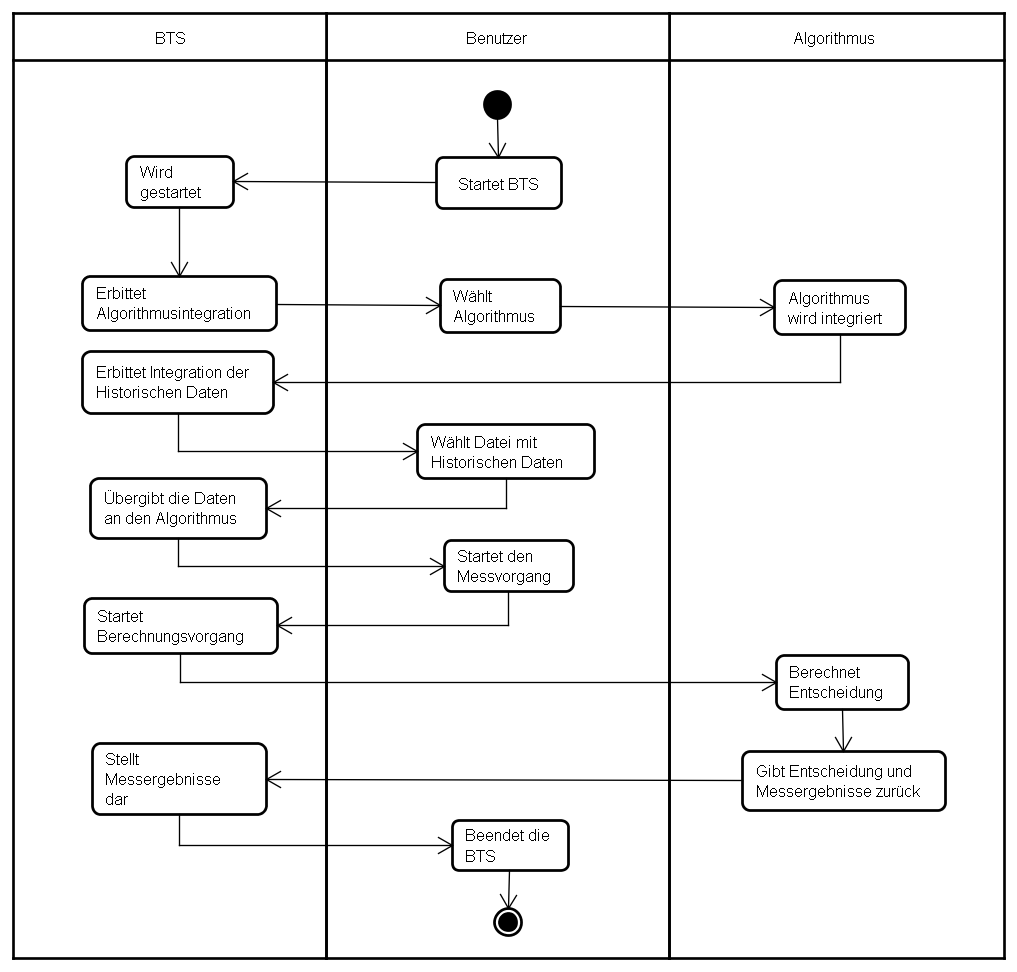
\includegraphics[width=1\textwidth]{graphics/Produktfunktionen/Standardabauf_1.png}
\captionof{figure}{Ein m�glicher Standardablauf von Noctua}}
\end{minipage}

